
%% siu_paper.tex
%% V1.3
%% 2007/01/11
%% by Michael Shell
%% See:
%% http://www.michaelshell.org/
%% for current contact information.
%%
%% This is a skeleton file demonstrating the use of IEEEtran.cls
%% (requires IEEEtran.cls version 1.7 or later) with an IEEE conference paper.
%%
%% Support sites:
%% http://www.michaelshell.org/tex/ieeetran/
%% http://www.ctan.org/tex-archive/macros/latex/contrib/IEEEtran/
%% and
%% http://www.ieee.org/

%%*************************************************************************
%% Legal Notice:
%% This code is offered as-is without any warranty either expressed or
%% implied; without even the implied warranty of MERCHANTABILITY or
%% FITNESS FOR A PARTICULAR PURPOSE!
%% User assumes all risk.
%% In no event shall IEEE or any contributor to this code be liable for
%% any damages or losses, including, but not limited to, incidental,
%% consequential, or any other damages, resulting from the use or misuse
%% of any information contained here.
%%
%% All comments are the opinions of their respective authors and are not
%% necessarily endorsed by the IEEE.
%%
%% This work is distributed under the LaTeX Project Public License (LPPL)
%% ( http://www.latex-project.org/ ) version 1.3, and may be freely used,
%% distributed and modified. A copy of the LPPL, version 1.3, is included
%% in the base LaTeX documentation of all distributions of LaTeX released
%% 2003/12/01 or later.
%% Retain all contribution notices and credits.
%% ** Modified files should be clearly indicated as such, including  **
%% ** renaming them and changing author support contact information. **
%%
%% File list of work: IEEEtran.cls, IEEEtran_HOWTO.pdf, bare_adv.tex,
%%                    bare_conf.tex, bare_jrnl.tex, bare_jrnl_compsoc.tex
%%*************************************************************************

% *** Authors should verify (and, if needed, correct) their LaTeX system  ***
% *** with the testflow diagnostic prior to trusting their LaTeX platform ***
% *** with production work. IEEE's font choices can trigger bugs that do  ***
% *** not appear when using other class files.                            ***
% The testflow support page is at:
% http://www.michaelshell.org/tex/testflow/



% Note that the a4paper option is mainly intended so that authors in
% countries using A4 can easily print to A4 and see how their papers will
% look in print - the typesetting of the document will not typically be
% affected with changes in paper size (but the bottom and side margins will).
% Use the testflow package mentioned above to verify correct handling of
% both paper sizes by the user's LaTeX system.
%
% Also note that the "draftcls" or "draftclsnofoot", not "draft", option
% should be used if it is desired that the figures are to be displayed in
% draft mode.
%
\documentclass[conference]{IEEEtran}
% Add the compsoc option for Computer Society conferences.
%
% If IEEEtran.cls has not been installed into the LaTeX system files,
% manually specify the path to it like:
% \documentclass[conference]{../sty/IEEEtran}

\IEEEoverridecommandlockouts

% Turkce karakterler icin.
\usepackage[english]{babel}
%\usepackage[utf8]{inputenc} % Kullanılan encodinge göre utf8 yerine latin5 de yazılabilir.
%\usepackage[T1]{fontenc}



% Some very useful LaTeX packages include:
% (uncomment the ones you want to load)


% *** MISC UTILITY PACKAGES ***
%
%\usepackage{ifpdf}
% Heiko Oberdiek's ifpdf.sty is very useful if you need conditional
% compilation based on whether the output is pdf or dvi.
% usage:
% \ifpdf
%   % pdf code
% \else
%   % dvi code
% \fi
% The latest version of ifpdf.sty can be obtained from:
% http://www.ctan.org/tex-archive/macros/latex/contrib/oberdiek/
% Also, note that IEEEtran.cls V1.7 and later provides a builtin
% \ifCLASSINFOpdf conditional that works the same way.
% When switching from latex to pdflatex and vice-versa, the compiler may
% have to be run twice to clear warning/error messages.






% *** CITATION PACKAGES ***
%
\usepackage{cite}
% cite.sty was written by Donald Arseneau
% V1.6 and later of IEEEtran pre-defines the format of the cite.sty package
% \cite{} output to follow that of IEEE. Loading the cite package will
% result in citation numbers being automatically sorted and properly
% "compressed/ranged". e.g., [1], [9], [2], [7], [5], [6] without using
% cite.sty will become [1], [2], [5]--[7], [9] using cite.sty. cite.sty's
% \cite will automatically add leading space, if needed. Use cite.sty's
% noadjust option (cite.sty V3.8 and later) if you want to turn this off.
% cite.sty is already installed on most LaTeX systems. Be sure and use
% version 4.0 (2003-05-27) and later if using hyperref.sty. cite.sty does
% not currently provide for hyperlinked citations.
% The latest version can be obtained at:
% http://www.ctan.org/tex-archive/macros/latex/contrib/cite/
% The documentation is contained in the cite.sty file itself.






% *** GRAPHICS RELATED PACKAGES ***
%
\ifCLASSINFOpdf
  \usepackage[pdftex]{graphicx}
  % declare the path(s) where your graphic files are
  % \graphicspath{{../pdf/}{../jpeg/}}
  % and their extensions so you won't have to specify these with
  % every instance of \includegraphics
  % \DeclareGraphicsExtensions{.pdf,.jpeg,.png}
\else
  % or other class option (dvipsone, dvipdf, if not using dvips). graphicx
  % will default to the driver specified in the system graphics.cfg if no
  % driver is specified.
  % \usepackage[dvips]{graphicx}
  % declare the path(s) where your graphic files are
  % \graphicspath{{../eps/}}
  % and their extensions so you won't have to specify these with
  % every instance of \includegraphics
  % \DeclareGraphicsExtensions{.eps}
\fi
% graphicx was written by David Carlisle and Sebastian Rahtz. It is
% required if you want graphics, photos, etc. graphicx.sty is already
% installed on most LaTeX systems. The latest version and documentation can
% be obtained at:
% http://www.ctan.org/tex-archive/macros/latex/required/graphics/
% Another good source of documentation is "Using Imported Graphics in
% LaTeX2e" by Keith Reckdahl which can be found as epslatex.ps or
% epslatex.pdf at: http://www.ctan.org/tex-archive/info/
%
% latex, and pdflatex in dvi mode, support graphics in encapsulated
% postscript (.eps) format. pdflatex in pdf mode supports graphics
% in .pdf, .jpeg, .png and .mps (metapost) formats. Users should ensure
% that all non-photo figures use a vector format (.eps, .pdf, .mps) and
% not a bitmapped formats (.jpeg, .png). IEEE frowns on bitmapped formats
% which can result in "jaggedy"/blurry rendering of lines and letters as
% well as large increases in file sizes.
%
% You can find documentation about the pdfTeX application at:
% http://www.tug.org/applications/pdftex





% *** MATH PACKAGES ***
%
\usepackage[cmex10]{amsmath}
% A popular package from the American Mathematical Society that provides
% many useful and powerful commands for dealing with mathematics. If using
% it, be sure to load this package with the cmex10 option to ensure that
% only type 1 fonts will utilized at all point sizes. Without this option,
% it is possible that some math symbols, particularly those within
% footnotes, will be rendered in bitmap form which will result in a
% document that can not be IEEE Xplore compliant!
%
% Also, note that the amsmath package sets \interdisplaylinepenalty to 10000
% thus preventing page breaks from occurring within multiline equations. Use:
%\interdisplaylinepenalty=2500
% after loading amsmath to restore such page breaks as IEEEtran.cls normally
% does. amsmath.sty is already installed on most LaTeX systems. The latest
% version and documentation can be obtained at:
% http://www.ctan.org/tex-archive/macros/latex/required/amslatex/math/





% *** SPECIALIZED LIST PACKAGES ***
%
%\usepackage{algorithmic}
% algorithmic.sty was written by Peter Williams and Rogerio Brito.
% This package provides an algorithmic environment fo describing algorithms.
% You can use the algorithmic environment in-text or within a figure
% environment to provide for a floating algorithm. Do NOT use the algorithm
% floating environment provided by algorithm.sty (by the same authors) or
% algorithm2e.sty (by Christophe Fiorio) as IEEE does not use dedicated
% algorithm float types and packages that provide these will not provide
% correct IEEE style captions. The latest version and documentation of
% algorithmic.sty can be obtained at:
% http://www.ctan.org/tex-archive/macros/latex/contrib/algorithms/
% There is also a support site at:
% http://algorithms.berlios.de/index.html
% Also of interest may be the (relatively newer and more customizable)
% algorithmicx.sty package by Szasz Janos:
% http://www.ctan.org/tex-archive/macros/latex/contrib/algorithmicx/




% *** ALIGNMENT PACKAGES ***
%
%\usepackage{array}
% Frank Mittelbach's and David Carlisle's array.sty patches and improves
% the standard LaTeX2e array and tabular environments to provide better
% appearance and additional user controls. As the default LaTeX2e table
% generation code is lacking to the point of almost being broken with
% respect to the quality of the end results, all users are strongly
% advised to use an enhanced (at the very least that provided by array.sty)
% set of table tools. array.sty is already installed on most systems. The
% latest version and documentation can be obtained at:
% http://www.ctan.org/tex-archive/macros/latex/required/tools/


%\usepackage{mdwmath}
%\usepackage{mdwtab}
% Also highly recommended is Mark Wooding's extremely powerful MDW tools,
% especially mdwmath.sty and mdwtab.sty which are used to format equations
% and tables, respectively. The MDWtools set is already installed on most
% LaTeX systems. The lastest version and documentation is available at:
% http://www.ctan.org/tex-archive/macros/latex/contrib/mdwtools/


% IEEEtran contains the IEEEeqnarray family of commands that can be used to
% generate multiline equations as well as matrices, tables, etc., of high
% quality.


%\usepackage{eqparbox}
% Also of notable interest is Scott Pakin's eqparbox package for creating
% (automatically sized) equal width boxes - aka "natural width parboxes".
% Available at:
% http://www.ctan.org/tex-archive/macros/latex/contrib/eqparbox/





% *** SUBFIGURE PACKAGES ***
%\usepackage[tight,footnotesize]{subfigure}
% subfigure.sty was written by Steven Douglas Cochran. This package makes it
% easy to put subfigures in your figures. e.g., "Figure 1a and 1b". For IEEE
% work, it is a good idea to load it with the tight package option to reduce
% the amount of white space around the subfigures. subfigure.sty is already
% installed on most LaTeX systems. The latest version and documentation can
% be obtained at:
% http://www.ctan.org/tex-archive/obsolete/macros/latex/contrib/subfigure/
% subfigure.sty has been superceeded by subfig.sty.



%\usepackage[caption=false]{caption}
%\usepackage[font=footnotesize]{subfig}
% subfig.sty, also written by Steven Douglas Cochran, is the modern
% replacement for subfigure.sty. However, subfig.sty requires and
% automatically loads Axel Sommerfeldt's caption.sty which will override
% IEEEtran.cls handling of captions and this will result in nonIEEE style
% figure/table captions. To prevent this problem, be sure and preload
% caption.sty with its "caption=false" package option. This is will preserve
% IEEEtran.cls handing of captions. Version 1.3 (2005/06/28) and later
% (recommended due to many improvements over 1.2) of subfig.sty supports
% the caption=false option directly:
%\usepackage[caption=false,font=footnotesize]{subfig}
%
% The latest version and documentation can be obtained at:
% http://www.ctan.org/tex-archive/macros/latex/contrib/subfig/
% The latest version and documentation of caption.sty can be obtained at:
% http://www.ctan.org/tex-archive/macros/latex/contrib/caption/




% *** FLOAT PACKAGES ***
%
%\usepackage{fixltx2e}
% fixltx2e, the successor to the earlier fix2col.sty, was written by
% Frank Mittelbach and David Carlisle. This package corrects a few problems
% in the LaTeX2e kernel, the most notable of which is that in current
% LaTeX2e releases, the ordering of single and double column floats is not
% guaranteed to be preserved. Thus, an unpatched LaTeX2e can allow a
% single column figure to be placed prior to an earlier double column
% figure. The latest version and documentation can be found at:
% http://www.ctan.org/tex-archive/macros/latex/base/



%\usepackage{stfloats}
% stfloats.sty was written by Sigitas Tolusis. This package gives LaTeX2e
% the ability to do double column floats at the bottom of the page as well
% as the top. (e.g., "\begin{figure*}[!b]" is not normally possible in
% LaTeX2e). It also provides a command:
%\fnbelowfloat
% to enable the placement of footnotes below bottom floats (the standard
% LaTeX2e kernel puts them above bottom floats). This is an invasive package
% which rewrites many portions of the LaTeX2e float routines. It may not work
% with other packages that modify the LaTeX2e float routines. The latest
% version and documentation can be obtained at:
% http://www.ctan.org/tex-archive/macros/latex/contrib/sttools/
% Documentation is contained in the stfloats.sty comments as well as in the
% presfull.pdf file. Do not use the stfloats baselinefloat ability as IEEE
% does not allow \baselineskip to stretch. Authors submitting work to the
% IEEE should note that IEEE rarely uses double column equations and
% that authors should try to avoid such use. Do not be tempted to use the
% cuted.sty or midfloat.sty packages (also by Sigitas Tolusis) as IEEE does
% not format its papers in such ways.





% *** PDF, URL AND HYPERLINK PACKAGES ***
%
%\usepackage{url}
% url.sty was written by Donald Arseneau. It provides better support for
% handling and breaking URLs. url.sty is already installed on most LaTeX
% systems. The latest version can be obtained at:
% http://www.ctan.org/tex-archive/macros/latex/contrib/misc/
% Read the url.sty source comments for usage information. Basically,
% \url{my_url_here}.

% *** Do not adjust lengths that control margins, column widths, etc. ***
% *** Do not use packages that alter fonts (such as pslatex).         ***
% There should be no need to do such things with IEEEtran.cls V1.6 and later.
% (Unless specifically asked to do so by the journal or conference you plan
% to submit to, of course. )
\usepackage{multirow}
\usepackage{array}
\usepackage[lofdepth,lotdepth]{subfig}

% correct bad hyphenation here
\hyphenation{op-tical net-works semi-conduc-tor}


\begin{document}

\IEEEpubid{\makebox[\columnwidth]{978-1-4799-4874-1/14/\$31.00 ©2015 IEEE\hfill}
\hspace{\columnsep}\makebox[\columnwidth]{}}

%
% paper title
% can use linebreaks \\ within to get better formatting as desired
\title{Comparison of Hard Vector Quantization and Sparse Coding Based Soft
Quantization for Spatial Pyramid Matching in Scene Classification Problems}

% author names and affiliations
% use a multiple column layout for up to three different
% affiliations
\author{\IEEEauthorblockN{Mustafa Sert}
\IEEEauthorblockA{Department of Computer Engineering\\
Baskent University\\
Ankara, Turkey\\
msert@baskent.edu.tr }
\and
\IEEEauthorblockN{Hilal Ergun}
\IEEEauthorblockA{Department of Computer Engineering\\
Baskent University\\
Ankara, Turkey\\
21020005@baskent.edu.tr }
}

% conference papers do not typically use \thanks and this command
% is locked out in conference mode. If really needed, such as for
% the acknowledgment of grants, issue a \IEEEoverridecommandlockouts
% after \documentclass

% for over three affiliations, or if they all won't fit within the width
% of the page, use this alternative format:
%
% use for special paper notices
%\IEEEspecialpapernotice{(Invited Paper)}




% make the title area
\maketitle

\begin{ozet}
Bu belge, SİU 2015 bildirisi hazırlamanız için bir taslak içermektedir. Bu sebeple lütfen taslaktaki başlık, özet ve diğer format stillerini kullanınız.  \textit{*Dikkat:  Bildiri Başlığında ve özetlerde sembol, özel ve matematiksel karakterler kullanmayınız.}
%\boldmath
\end{ozet}
\begin{IEEEanahtar}
döküman biçimi, stil, anahtar kelimeler.
\end{IEEEanahtar}

\begin{abstract}
This electronic document is a “live” template and already defines the components of your paper [title, text, heads, etc.] in its style sheet.  \textit{*CRITICAL:  Do Not Use Symbols, Special Characters, or Math in Paper Title or Abstract.}
%\boldmath
\end{abstract}
\begin{IEEEkeywords}
component, formatting, style, styling, insert (key words).
\end{IEEEkeywords}

% IEEEtran.cls defaults to using nonbold math in the Abstract.
% This preserves the distinction between vectors and scalars. However,
% if the conference you are submitting to favors bold math in the abstract,
% then you can use LaTeX's standard command \boldmath at the very start
% of the abstract to achieve this. Many IEEE journals/conferences frown on
% math in the abstract anyway.

% no keywords

% For peer review papers, you can put extra information on the cover
% page as needed:
% \ifCLASSOPTIONpeerreview
% \begin{center} \bfseries EDICS Category: 3-BBND \end{center}
% \fi
%
% For peerreview papers, this IEEEtran command inserts a page break and
% creates the second title. It will be ignored for other modes.
\IEEEpeerreviewmaketitle

\IEEEpubidadjcol

\section{Introduction}

Image scene classification is one the difficult problems of image processing community. Mostly attributed to semantic gap phenomenon, classification of images or scenes by computer programs into meaningful categories which can be resolved by humans natively is a non-trivial problem. Intra-class variation, clutter, occlusion, different poses of same objects add up to obstacles waiting to be overcome~\cite{LocalFeaturesAndKernels}. Artificial algorithms  should be able to match local or global image features to the semantic categories defined for the image. However, describing semantic categories in terms of image features is not a straightforward task.

The recognition of texture and object categories is one of the most challenging problems in computer vision, especially in the presence of intra-class varia- tion, clutter, occlusion, and pose changes[7]

Bag of words algorithm is one the most succesful approaches which can, to some extent, fill semantic gap between high level image categories and image features. Bag of words algorithm finds its roots in the document classification domain. In very simple terms, bag-of-words approach counts occurrence of local image features and tries to represent higher level image categories using this information. In their very simple form, bag-of-features methods discard all spatial information present in the image and retain only the visual words' visibility frequencies~\cite{LocalFeaturesAndKernels}.

One of the possible extensions to classical bag-of-words model is to use of spatial pyramids. In this approach, image is divided into smaller images and bag-of-words model is independently applied to each smaller image. Later, these finer-grained image histogramds are concatanated to create final image representation. Spatial pyramids provide a good cover for the spatial space and many state-of-the-art classification implementations use them of modified versions~\cite{6248076}.

Bag of features approach for local features based image classification has long been proved to be a very successful implementation. Inserting spatial pyramids to the processing pipelines is another succesful approach for reaching higher classification rates. However, further classification performance increase using using spatial pyramids alone seems unlikely. Recent studies tries to overcome limititions using better feature quantization techniques. Using sparse coding techinques has been showing promising results on the image classification datasets.

Bag-of-words model can be represented with four image processing steps. First, image features are calculated for target images. Different local image features can be used at this step, SIFT being one of the most popular choices. Furthermore, more than one type of image features can be extracted. After image feature extraction comes the quantization step. In this step, image features are quantized or assigned into different bag-of-words dictionary bins. Hard or soft assigment may be employed in this step. Vector quantiziation is the mostly employed hard assignment techinque. Gaussian mixture models and sparse coding being mostly used soft assignment techinques. Later comes the pooling stage. In this step quantized image features are pooled to create global image representation which can be called bag-of-words descriptor for the given image. Last and forth step is the classification of bag-of-words descriptor. Different machine learning approaches may be used in this step, support vector machines being most frequently used classifiers in the literature.

[Neden vector quantization ve sparse coding karsilastiriyoruz bundan bahsedelim.]

In this work we will compare performance of sparse codes based soft assignment and vector quantization of SIFT features. We will use 3 different benchmark databases for comparison.

\section {Related Work}

In a typical BoW based image classification pipeline, 4 distinct operations performed on images~\cite{6248076}~\cite{5206757}. Local images features are extracted as a first step. Later on, these features are encoded in a more suitable manner for classification. In the third step encoded features are pooled to create final image representation by summarizing coded features over larger neighborhoods. In the last step, image representing descriptors is classified using a suitable classifier. This process is outlined in Figure 1.

\begin{figure}[h]
\centering
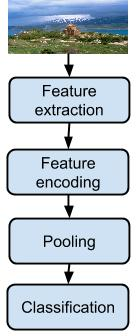
\includegraphics[scale=0.5]{data/classification_pipeline.jpg}
\caption{Classification pipeline overview}
\label{figure1}
\end{figure}

\subsection{Feature Extraction}

Many papers show that dense feature extraction outperforms interest-point based extraction on visual classification tasks~\cite{1641019},~\cite{1541309}.

\subsection{Encoding}

Feature encoding, or coding, is the process of re-coding image descriptors to a different representation. Encoding step does not alter the local nature of the image features, each feature is transformed locally by transforming descriptors pointwise~\cite{5539963}. This encoding process aims to derive a more suitable feature representation for classification process.

One alternative to overcome high quantization errors induced by vector quantization is to use soft-assignment codings. Gemert et al. reaches a soft-assignment coding by introducing uncertainty into vector quantization~\cite{5128909}. They also investigate possible other soft-assigment strategies and emphasize the success uncertainty modelling. They investigate previous papers using feature distances for assigning multiple codewords to single local feature. Feature space partioning approaches improves encodings locality which is a desired property for upper layers in the classification pipeline~\cite{Avila2013453}. We will visit locality later in pooling section.

Sparse coding has some attractive properties when compared to vector quantization(VQ). One of them is sparse coding(SC) has a lower reconstruction error. This can be easily verified by comparing vectoral representations of both VQ and SC. VQ has a binary representation where each cell of encoded representation is represented either by ones of zeros whereas SC assigns continious values to vector cells. One should note that SC uses more bits to represent local feature even VQ and SC uses same dictionary sizes. Another attractive property of SC is that it better captures salient properties of images. Furthermore, image patches are better represented with sparse signals~\cite{5539963}. Furthermore, sparsity in the representation helps classification esspecially when linear classifiers are used\cite{6248076}.

Encoding process may be skipped in total if computationally more advanced pooling strategies are used. One example is ~\cite{SecondOrderPooling} where authors prefer not to encode raw SIFT descriptors but use as is in the pooling step.

\subsection {Pooling}

Pooling can be defined as the operation which creates global image representation from underlying local feature encodings\cite{6248076}. Roots of feature pooling concept can be found in very early studies dating back to 1960's and attributed mostly to the concept of locally orderless images~\cite{boureau2010theoretical}. Pooling aggregates local encodings into a more compact representation. Due to this compacting nature, it may lead to information loss as well as some form of invariance to feature perturbations~\cite{6909713}. Lazebnik et al. showed finer grained pooling using spatial pyramids on top of generic bag-of-features implementations ~\cite{1238663} yields better classification results. Wang et al. offered a different local pooling strategy which may furher improve classification results on top of spatial pyramids~\cite{5540018}. Several other pooling methodologies are offered in various papers~\cite{Avila2013453},~\cite{6126555},~\cite{ObjectCentricPooling},~\cite{6248076},~\cite{SecondOrderPooling}. In their theoretical analysis of feature pooling~\cite{boureau2010theoretical}, Boureu et al. argue that using all samples may not be optimal and pooling close descriptors either in feature space or spatial domain may yield better results~\cite{6909713}.

Among several different poolings strategies present in the literature, we are interested in two of which attracted most attention. One of them is summed or average pooling which yields a histogram like representation~\cite{5539963} and the other is maximum pooling. Pooling operator takes activations in a certain spatial region to create each dimension global pooled feature\cite{6248076}.

Maximum spatial pooling is said to be more robust to spatial translations than the average pooling~\cite{5206757}. Max pooling is attributed to be more biological plausible and inspired by several authors. However, we found this argument as a debatable one. We know that both max and average pooling are employed in several stages of visual cortex~\cite{6909713}. On the other hand, this doesn't prevent max pooling being a very good pooling strategy, beating average pooling in various configurations~\cite{5539963}. Intiuatively unexpected success of max pooling can be explained by it being more salient and robust to local translations~\cite{5539963}.

In addition to direct maximum and average pooling approaches, several implementations suggest using modified alternatives. ~\cite{Avila2013453} uses feature distribution around each codeword in addition to average pooling. They employ a non-parametric estimation techinque for feature distribution. However, we should note that one must take into consideration while applying distribution based techniques that most frequent features are not always the most discriminative ones~\cite{5128909}.


~\cite{McCannL12} suggests using of totally different 

\subsection {Classification}

Support vector machines(SVMs) are one of the mostly adapted,if not the most, classifiers in the literature for the task of classifing final image representation. 

Different non-linear and linear kernels employed for classification of different representations. Nonlinear SVMs are known to have higher complexity than linear SVMs ~\cite{5206757} and they are not preferred for large image databases.

When using vector quantization, linear kernels deliver substantially worse results~\cite{1641019}~\cite{5539963} Yang et al. states this is due to high quantization error in encoding step.

Among non-linear kernels we found chi2 and histogram interection kernels to be most useful. One other choice frequently used in the literature is the Earth's mover distance kernel, namely EMD kernel. However, previous work showed that performance of EMD is comparable with chi2~\cite{LocalFeaturesAndKernels} so we don't use EMD at all.

\section {Experimental Results}

\subsection {State-of-the-art}

~\cite{SecondOrderPooling} : comparison: \%79 performance at multiple scales and 4 point step size, \%70 performance at single scale and 8 point step size. We do \%77 at multiple scales.

\subsection {Dictionary construction}
\subsection {Feature extraction}
In this work we will not look into details of feature extraction methodologies. One can employ different feature types, sampling strategies, multi-scale extraction, multi-feature approaches during feature extraction. In our work we will investigate performance of one type image feature, SIFT features. Our features will be extracted in a single scale with dense sampling strategy.[Bu results icin daha mi uygun acaba?]
\subsection {Feature encoding}

\subsection {Pooling}

Note1: as well as geometric lp norm pooling, mix-order max pooling is suggested by people.

\clearpage

\section{RESULTS}

\subsection{Caltech 101}

[Caltech 101'i anlat, veri seciminden bahset]

\begin{table}[ph]
  \centering
  \begin{tabular}{|c|c|c|c|}
    \hline
    \multirow{2}{*}{Dictionary Sizes} & \multicolumn{3}{c|}{Classification Accuracy} \\
    \cline{2-4}
    & SPM & ScSPM & LLC \\
    \hline
     L2, K=1024 & & & \\
    \hline
     L2, K=1024 & & & \\
    \hline
  \end{tabular}
  \caption{Classification accuracy on Caltech-101 dataset }
  \label{tablo}
\end{table}

\subsection{Caltech 256} 

[Caltech 256'i anlat, veri seciminden bahset]

\begin{table}[ph]
  \centering
  \begin{tabular}{|c|c|c|c|}
    \hline
    \multirow{2}{*}{Dictionary Sizes} & \multicolumn{3}{c|}{Classification Accuracy} \\
    \cline{2-4}
    & SPM & ScSPM & LLC \\
    \hline
     L2, K=1024 & & & \\
    \hline
     L2, K=1024 & & & \\
    \hline
  \end{tabular}
  \caption{Classification accuracy on Caltech-256 dataset }
  \label{tablo}
\end{table}

\subsection{Pascal VOC 2007}

Burada Pascal VOC 2007 anlatalim.

\begin{table}[ph]
  \centering
  \begin{tabular}{|c|c|c|}
    \hline
    \multirow{2}{*}{Dictionary Sizes} & \multicolumn{2}{c|}{mAP} \\
    \cline{2-3}
    & \ SPM\ \ & ScSPM \\
    \hline
     K=128 & 0.2205 & 0.2337 \\
    \hline
     K=256 & 0.2294 & 0.2786 \\
     \hline
     K=512 & 0.2370 & 0.3164 \\
     \hline
     K=1024 & 0.2450 & 0.3486 \\
     \hline
     K=2048 & & 0.3783 \\
     \hline
     K=4096 & & \\
    \hline
  \end{tabular}
  \caption{ mAP on VOC 2007 challenge dataset }
  \label{tablo}
\end{table}

\begin{table}[ph]
  \centering
  \begin{tabular}{|c|c|c|}
    \hline
    \multirow{2}{*}{Image Categories} & \multicolumn{2}{c|}{mAP} \\
    \cline{2-3}
               & \ SPM\ \ & ScSPM \\
    \hline
     Aeroplane & 0.5010 & 0.6332 \\
    \hline
     Bicycle & 0.2319 & 0.4333 \\
     \hline
     Bird & 0.1909 & 0.3705 \\
     \hline
     Boat & 0.2948 & 0.4366 \\
     \hline
     Bottle & 0.0933 & 0.1686 \\
     \hline
     Bus & 0.2014 & 0.3659 \\
     \hline
     Car & 0.4029 & 0.5898 \\
     \hline
     Cat & 0.3098 & 0.4377 \\
     \hline
     Chair & 0.0856 & 0.0992 \\
     \hline
     Cow & 0.1191 & 0.1979 \\
     \hline
     Dining Table & 0.2218 & 0.4118 \\
     \hline
     Dog & 0.1998 & 0.3047 \\
     \hline
     Horse & 0.4600 & 0.5694 \\
     \hline
     Motorbike & 0.2647 & 0.4402 \\
     \hline
     Person & 0.2850 & 0.4088 \\
    \hline
     Pottedplant & 0.0691 & 0.1623 \\
     \hline
     Sheep & 0.1704 & 0.2620 \\
     \hline
     Sofa & 0.1455 & 0.3335 \\
     \hline
     Train & 0,4709 & 0.6107 \\
     \hline
     TV/Monitor & 0.1813 & 0.3295 \\
     \hline
  \end{tabular}
  \caption{ ScSPM=2048 SPM=1024 }
  \label{tablo}
\end{table}

% no \IEEEPARstart

% You must have at least 2 lines in the paragraph with the drop letter

% (should never be an issue)

\bibliographystyle{plain}
\bibliography{siu_paper}

% that's all folks
\end{document}


